\documentclass[12pt]{article}
\usepackage[utf8]{inputenc}
\usepackage{graphicx} 
\usepackage{wrapfig}
\usepackage[dvipsnames]{xcolor}
\usepackage{moreverb}
\usepackage{ragged2e}
\renewcommand\refname{Referencias}
\title{Elementos de la programación Python 1.}
\author{\textcolor{JungleGreen}{Olga María Fimbres Morales}}
\date{28 de Enero 2016}
\begin{document}
\begin{titlepage}

\begin{center}
\begin{large}
Universidad del Estado de Sonora\\
\end{large}
\vspace*{0.15in}
División de Ciencias Exactas y Naturales.\\
\vspace*{0.15in}
Licenciatura en Física. \\
\vspace*{0.6in}
\begin{large}
Física Computacional 1\\
\end{large}
\vspace*{0.2in}
\begin{Large}
\textbf{{\textcolor{Red}{Periodo del Péndulo.}}} \\
\end{Large}

%\begin{Large}
%\textbf{{\textcolor{Red}{Péndulo.}}} \\
%end{Large}
%\vspace*{-1in}

\rule{80mm}{0.1mm}\\
\vspace*{0.1in}
\begin{large}
{\textcolor{JungleGreen}{Olga María Fimbres Morales}}\\
14 de Marzo de 2016\\
\end{large}
\end{center}
\end{titlepage}

\pagebreak
\section*{Introducción.}
 Como ya se ha abordado anteriormente, sabemos que el sistema físico del péndulo resulta mas complejo conforme los ángulos entre los que se maneje aumenten de aquellos para los que funciona el modelo del péndulo simple.\\
 Sabemos que su solución resulta muy diferente entre ambos escenarios y evidentemente podemos observar que habrá una diferencia entre sus periodos, siendo mas complejo el periodo para el péndulo de ángulos mayores.\\
 Durante esta actividad, se realizo un pequeño análisis sobre que ocurre al cambiar de un sistema de péndulo simple a uno mas complejo en relación a los periodos y el error que existe entre ambos; permitiéndonos observar cual resulta más adecuado para cada situación.
 
 
\section*{\textcolor{Red}{Péndulo}}
\begin{wrapfigure}{r}{6cm}
	\begin{center}
      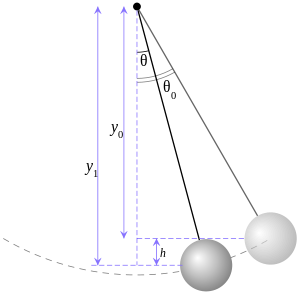
\includegraphics[width=6.0cm]{pendulo.png}
      \caption{Péndulo simple \cite{Img1}.}
    \end{center}
\end{wrapfigure}
Al haber estudiado este sistema con anterioridad ya es de nuestro conocimiento el sistema idealizado del péndulo simple y las características que los identifican como tal, es decir:
\begin{itemize}
\item Cordón rígido.
\item Masa puntual.
\item El movimiento que describe es el de un arco.
\item Su energía se conserva, es decir, no existe fricción.
\end{itemize}

Recordemos, que este modelo solo funciona para ángulos pequeños, es decir aquellos que tienen como máximo, aproximadamente, 30 grados.
\pagebreak
\subsection*{\textcolor{NavyBlue}{Periodo para ángulos pequeños.}}
Mientras nos encontremos trabajando con ángulos menores a los 30 grados, podremos definir el periodo del péndulo de la siguiente forma:
\begin{eqnarray*}
\textcolor{Emerald}{T = 2\pi \sqrt{\frac{l}{g}}}
\end{eqnarray*}

Expresión que obtenemos de la solución de la ecuación diferencial para el péndulo simple con condiciones iniciales adecuadas.\\
Dicha expresión de conoce como la ley del periodo de Christiaan Huygens; de donde se puede observar fácilmente que este resulta independiente de la amplitud $\theta_0$, siendo esta una cualidad más del péndulo simple, ya que sin importar su ángulo inicial su periodo sera el mismo y solamente se vera afectado al cambiar la longitud de la cuerda.\\

\subsection*{\textcolor{NavyBlue}{Amplitudes arbitrarias.}}
Tal como hemos visto en actividades anteriores la complejidad del cálculo del periodo para este tipo de péndulos es tal que resulta necesaria la utilización de una herramienta computacional para realizar una serie de integrales e invirtiendo la ecuación, obtenida a partir de la energía, para la velocidad angular:

\begin{eqnarray*}
\frac{dt}{d \theta} = \sqrt{\frac{l}{2g}} \frac{1}{\sqrt{\cos\theta -  \cos\theta_0}}
\end{eqnarray*}

y después integrando sobre un ciclo completo
\begin{eqnarray*}
T = t(\theta_0 \to 0 \to -\theta_0 \to 0 \to \theta_0)
\end{eqnarray*}

o dos veces un medio ciclo
\begin{eqnarray*}
T=2t(\theta_0 \to 0 \to -\theta_0)
\end{eqnarray*}

o cuatro veces un cuarto de ciclo
\begin{eqnarray*}
T=4t(\theta_0 \to 0)
\end{eqnarray*}

lo cual nos lleva a
\begin{eqnarray*}
\textcolor{Emerald}{T=4 \sqrt{\frac{l}{2g}}\int\limits_0^{\theta_0} \frac{1}{\sqrt{\cos\theta - \cos\theta_0}} d\theta}
\end{eqnarray*}


\pagebreak
\section*{\textcolor{LimeGreen}{Problema.}}
Esta vez, la actividad que se pidió realizar es un análisis en la diferencia del cálculo del periodo del péndulo para ángulos entre 0 y $\pi$ de la forma en que se hace para el péndulo simple y de la forma para ángulos arbitrarios.\\
Se utilizó la herramienta $odeint$ de Python estudiada en la actividad anterior para realizar las integrales pertinentes para nuestro escenario.\\

Inicialmente de especifican las herramientas que se utilizaran en el programa, para nuestro código utilizaremos la herramienta anteriormente mencionada, numpy y matplotlib pues se buscar tener como resultado una gráfica de los errores.\\

En seguida se especifican las variables necesarias para conocer el periodo para el caso del péndulo simple, para lo cual solamente necesitamos la aceleración de la gravedad y la longitud de la cuerda, la que en este caso se decidió fuera de 1 metro. Una vez que se tienen estas variables se calcula el periodo correspondiente y se le conoce como $T_o$.\\

A continuación se calcula el periodo para el caso de ángulos arbitrarios, que a simple vista podemos decir es más complicado que el periodo calculado anteriormente. En un inicio es necesario definir nuestra función la cual dependerá del parámetro $\theta$. Enseguida se inicia el ciclo para integrar, definiendo como punto de partida un $\theta_0 = 0$ y como condición que este sea menor a $\pi$, sin embargo, si esto es dejado solamente de esta forma el programa presenta un error y el último dato generado resulta ser no numérico; por lo que es necesario restarle una pequeña cantidad como limite, lo cual se especifica en la condición. Ahora es necesario definir la forma en que esta ira variando, para lo cual a cada $\theta_0$ anterior se le suma 0.05.\\

Una vez terminado este ciclo, se realiza la integración de nuestra función anteriormente especificada con limite inferior 0 y superior la secuencia de números obtenidos para $\theta_0$.\\

Finalmente se realiza la gráfica correspondiente $\theta_0 vs \frac{T}{T_0}$. Realizando las especificaciones que se consideren adecuadas tanto para el formato como para el estilo deseado de la gráfica resultado.

\begin{boxedverbatim}
from scipy import integrate
import numpy as np
import matplotlib.pyplot as plt

l = 1. #longitud de la cuerda
g = 9.81

#periodo para oscilaciones pequeñas
To = 2*np.pi*sqrt(l/g) 

#periodo para oscilaciones arbitrarias
#definir la función a integrar

#theta_0 = np.linspace(0, np.pi-0.001 ,100)

X = lambda theta: 1.0/(np.sqrt(np.cos(theta)-np.cos(theta_0)))
#ciclo para integrar
theta_0 = 0.0
while (theta_0 < np.pi-0.08): 
#es necesario restringirlo a un numero antes de pi, 
pero si este es muy pequeño 
el programa tiene problemas para correr
    theta_0 = theta_0 + 0.05
    int2 = integrate.quad(X, 0.0, theta_0)    
    
    #print(int2[0])
    #theta = (theta_0*360)/np.pi
    #print(theta)
    T = 4*sqrt(l/(2*g))*int2[0]
    #print(T)
    Z = T/To
    #print(Z)
    #print(theta_0)
    plt.plot(theta_0 ,Z,'o', label='Error relativo')
    plt.grid(True)
    plt.xlabel('Theta',fontsize=15)
    plt.ylabel('T/To',fontsize=15)
    v=[0,np.pi/2,1,1.2]
    axis(v)
    #plt.legend()
    #plt.show()
\end{boxedverbatim}





\pagebreak

\section*{\textcolor{RoyalBlue}{Resultados}}
Una vez que el código trabaja de la manera adecuada nos arroja la gráfica correspondiente al error relativo que existe entre utilizar el calculo del periodo considerando un péndulo simple o considerando un péndulo para cualquier amplitud de ángulos.

\begin{center}
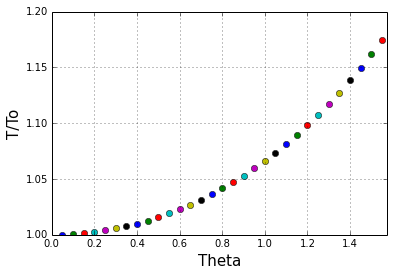
\includegraphics{actividad6.png}
\end{center}

De esto podemos observar que a medida que la amplitud del ángulo inicial en un péndulo aumenta la diferencia entre los resultados arrojados por cada uno de las escenarios aumenta significativamente, por lo que la indiferencia de utilizar una formula o la otra solamente es aceptada {content...}para amplitudes pequeñas menores, aproximadamente, de los 0.4 radianes es decir cerca de 23 grados.\\

Una vez superado esa amplitud el problema debe ser tratado de la forma correspondiente o se estará generando un dato con un importante error, lo cual puede perjudicar nuestros estudios del fenómeno.

\pagebreak
\begin{thebibliography}{X}
 \bibitem{1} \textsc{Wikipedia, The free encyclopedia; "Pendulum"; 2016}{content...}
 \bibitem{Wik} \textsc{Wikipedia, The free encyclopedia; "Pendulum (mathematics)"; 2016}
 \bibitem{Img1} \textsc{By Krishnavedala; via Wikimedia Commons;"Pendulum (mathematics)"}
 \bibitem{5} \textsc{scipy.integrate.odeint de Python}
\end{thebibliography}
\end{document}